\documentclass[preprint,11pt]{sigplanconf}
\usepackage[colorlinks=true,linkcolor=black,urlcolor=black,citecolor=black]%
{hyperref}
\usepackage{graphicx}
\usepackage{verbatim}
\newenvironment{smallverbatim}{\endgraf\small\verbatim}{\endverbatim} 
\renewcommand{\t}{\texttt}
\renewcommand{\b}{\textbf}
\renewcommand{\i}{\textit}

\newcommand{\prettybox}[1]{\fbox{\parbox{\linewidth}{#1}}}

% A bunch of crazy BNF TeX I wrote once
\def\bnf#1{\prettybox{\halign{##\hfil& \hfil ##\hfil& \ ##\hfil\cr #1}}}
\def\p#1{& = & #1 \cr}
\def\pp#1{& & #1 \cr}
\def\a#1{& $\mid$ & #1 \cr}

\title{He-Man: A domain-specific language for lightweight concurrency}
%\subtitle{I said hey, what's goin' on}
\authorinfo{Carlo Angiuli}{}{cangiuli@cs.cmu.edu}
\authorinfo{Michael Sullivan}{}{mjsulliv@andrew.cmu.edu}
\date{December 12, 2011}

\begin{document}
\maketitle

\begin{abstract}
TODO
\end{abstract}

\section{Introduction}

Network applications need to support many simultaneous clients---this is known
as the C10K (``10,000 client'') problem \cite{Kegel}. Modern servers have enough
memory and bandwidth for massive concurrency, but it is difficult to design
applications to take full advantage of these resources.

A server must maintain separate state for each connection, and often waits for
network or disk I/O to complete before continuing to serve a particular client.
The simplest solution is to maintain one thread per client, using blocking I/O
within each thread. This incurs frequent and expensive context switches at the
operating system level; because the threads have identical code and little
private data, this approach is unnecessary and does not scale.

An improvement is to write multithreaded code, in which each thread serves
multiple clients. This is the most popular approach, and is utilized in the
Apache HTTP server \cite{Apache}.

Languages like Erlang and Haskell provide lightweight threads via user-space
schedulers. This affords even better performance, but remains unnecessarily
powerful for this problem space, imposing runtime overhead on applications which
don't require preemptable, independently scheduled threads \cite{Vinoski}.

By far the leanest approach is to write an event loop around kernel facilities
for multiplexed, non-blocking I/O, such as \t{select}, \t{poll}, \t{epoll}, or
\t{kquery}. In this model, all blocking occurs at a single call site in the
code. The programmer is responsible for explicitly maintaining per-client state
and invoking the appropriate client on each I/O event.

This requires the entire application to be restructured as a state machine with
explicit per-client control blocks, a model which is very difficult for
programmers to reason about. There exist numerous C/C++ libraries for event
loops, but none of these avoid the state machine paradigm.

Our observation is that the event loop model, in programming languages parlance,
is essentially trampolining continuation-passing-style, which can be obtained by
mechanical translation from the straight-line threaded code. This suggests it is
possible to obtain the best of both worlds---a threaded programming model with
the performance of event loops. 

To that end, we present He-Man: Haskell Event Manager, Apropos Networking, an
embedded domain-specific language (EDSL) hosted in Haskell, which provides a
threaded abstraction for network application programming and compiles to a C
event loop based around Linux's \t{epoll}.

He-Man is a straightforward monadic language with built-in network primitives,
offering a simple thread-per-client programming model. It is easily extensible
in Haskell, and also allows calls to foreign C functions; it outputs C code
which links with an event loop runtime and any code a programmer might prefer to
write directly in C. Our vision is that C programmers can use He-Man for their
core application logic, and can write the rest of their application in C. 

\section{Related work}

The C10K problem is particularly evident in the context of HTTP servers, which
routinely maintain many concurrent connections. As we discuss in Section
\ref{sec:evaluation}, Apache does not scale particularly well. The popular
Lighttpd and Nginx HTTP server projects were both started with the explicit goal
of outperforming Apache with respect to the C10K problem \cite{Lighttpd,Nginx},
and both use event-based architectures similar to He-Man. 

A number of functional languages support lightweight threads with user-space
scheduling, most notably Erlang, which was designed for highly concurrent
telecommunications applications, and easily scales to 20,000 clients
\cite{Hellstrom}. The Haskell runtime supports a variety of concurrency
primitives which permit a lightweight threaded programming model \cite{LiEtAl}.

%A number of custom network stack implementations exist for functional
%languages, such as FoxNet for Standard ML \cite{BiagioniEtAl}, and 

He-Man is most similar to Li and Zdancewic's Haskell implementation of a hybrid
event/thread programming model for network applications \cite{LiZdancewic}.
Their project has similar goals to ours, but is implemented entirely within
Haskell. As a result, unlike He-Man, their framework requires entire
applications to be written in Haskell, and incurs runtime overhead from the
Haskell system.

\section{The event loop model}

Networking applications require a very constrained form of concurrency. Because
I/O (both network and disk) latency dominates the computation time, each
client's thread of execution spends most of its time waiting on I/O. In
particular, we would like to always yield to a client no longer blocked on I/O;
we need not yield to blocked clients, nor do we need arbitrary interleaving of
execution.

As of version 2.5.44, Linux has supported \t{epoll} for non-blocking
multiplexing I/O. A server can register any number of file descriptors with
\t{epoll\_ctl}, and a call to \t{epoll\_wait} returns the ready descriptors. 

In the event loop model, all blocking I/O must occur in a single loop around
\t{epoll\_wait}. Each thread is stored as a \t{struct} containing thread-local
state, including the next instruction pointer, and each registered descriptor
has a pointer to the thread waiting on it. Instead of performing an I/O call, a
thread simply registers a new descriptor and returns back to the main loop;
whenever a descriptor is ready, the main loop jumps to the instruction pointer
of the thread waiting on it. Spawning a new thread requires only allocating a
new thread \t{struct}, and registering it in the main loop.

Each thread must be split into one function for each jump target, and
thread-local state must be accessed via the thread \t{struct} shared between
these functions. Furthermore, because I/O only occurs in the main loop, these
functions must return immediately after registering new descriptors. As a
result, each thread is split up into quite a few functions in this paradigm.
Because this translation from threaded to event-based is quite mechanical, we
are able to perform it automatically in the He-Man back-end.

\section{Implementation}

\subsection{Front-end}

The underlying abstract syntax for the front-end He-Man language is a
fairly conventional imperative, statement based, first order language,
shown in Figure \ref{fig:front-syntax}. The notable constructs are
\b{Spawn}, which creates a new thread that takes a list of arguments
and launches the associated code with those arguments available to it,
and \b{Wait}, which takes an event expression as an argument and
blocks until the event has ``completed''. Note that \b{Call} is for
calling foreign functions; He-Man does not have its own notion of
function.

Since writing programs using the abstract syntax would be highly
inconvenient, we provide a monadic library for writing He-Man
programs, which allows us to leverage Haskell's do notation to write
He-Man programs using convenient imperative syntax. In this way, we
are taking advantage of monads being ``programmable semi-colons''.

We define the \t{Prog} monad, which contains a \t{State} monad used to
maintain a counter for generating unique variable names and a
\t{Writer} monad that is used to build up a list of statements. We
then provide \t{Prog} wrappers for statements that add the statement
to the list of statements being built up by the \t{Writer}. The
wrappers for \b{Spawn}, \b{Assign}, \b{Wait}, and \b{Exit} simply take
the obvious arguments, construct a \t{Stmt} and add it to the writer
list. The \b{Assign} wrapper is an infix operator, and is named
``.=''. The wrappers for \b{While} and \b{If} take values in \t{Prog}
instead of statement lists, and run the \t{Writer} to extract the
lists of statements. The monadic wrapper for \b{Decl} declares a
variable (with a name made unique by appending a unique number) and
then returns the \t{Expr} that references the declared variables. This
makes declaring and using variables very natural. We also provide a
wrapper for \b{Call} that declares a fresh variable, assigns the
result of a call to it, and then returns the variable. Then,
``declaring'' a foreign function consists of writing a convenient
wrapper function that invokes the \b{Call} wrapper.

At the expression level, \t{Expr} is an instance of the \t{Num} type
class so that numeric literals and operations can be used in He-Man
syntax. We also provide infix operators for other useful operations on
expressions, some of them with mildly awkward names, since the good
names were already taken by a function with the wrong type.

The result of all of this is that He-Man code can be written in a
fairly natural style, as shown in Figure \ref{fig:code-ex}.

Although the He-Man target language does not support defining
functions, code modularity and reuse is easily supported while writing
He-Man code by defining Haskell functions that produce values in
\t{Prog}. When invoked, the code of these meta-level ``functions'' is
included directly at the call-site. This is a very powerful tool, but
can potentially result in code size explosion if used carelessly.

As an example of the power that Haskell and the monadic style gives
us, Figure \ref{fig:generic} shows our library routines for simulating
blocking network operations. \t{do\_nb\_action} takes an event
\t{Expr} and a \t{Prog Expr} action representing a network call that
can return \t{EAGAIN} and produces an action that generates code to
simulate a blocking network operation. This allows us to describe how
to simulate blocking I/O in a generic way, and then invoke it to
create our concrete wrappers.
(\t{.=.} is a wrapper for
\b{Assign} that takes a \t{Prog Expr} as its second argument and the
\t{sock\_*} functions invoke \b{Call} wrappers on the appropriate
network calls).

\begin{figure}[ht]
\centering
\bnf{
\i{Stmt}
\p{\b{Decl} (\i{Var}, \i{Type}) \i{Expr}}
\a{\b{While} \i{Expr} [\i{Stmt}]}
\a{\b{If} \i{Expr} [\i{Stmt}] [\i{Stmt}]}
\a{\b{Spawn} ([(\i{Var}, \i{Type})], [\i{Stmt}]) [\i{Expr}]}
\a{\b{Assign} \i{Expr} \i{Expr}}
\a{\b{Exp} \i{Expr}}
\a{\b{Wait} \i{Expr}}
\a{\b{Exit}}
\i{Expr}
\p{\b{Call} \i{String} [\i{Expr}]}
\a{\b{Arith} \i{ArithOp} \i{Expr} \i{Expr}}
\a{\b{ArithUnop} \i{ArithUnop} \i{Expr}}
\a{\b{RelnOp} \i{RelnOp} \i{Expr} \i{Expr}}
\a{\b{Constant} \i{String}}
\a{\b{NumLit} \i{Integer}}
\a{\b{StringLit} \i{String}}
\a{\b{Var} \i{String}}
\a{\b{CurThread}}
\i{Type} 
\p{\b{Int} $\mid$ \b{Bool} $\mid$ \b{String}
   $\mid$ \b{Buffer} $\mid$ \b{Event}}
}
\caption{Front-end grammar.}
\label{fig:front-syntax}
\end{figure}

\begin{figure}[ht]
\centering
\begin{smallverbatim}
child_code = declare_thread [("child_fd", Int)] $
  \[child_fd] -> do
  ev <- setup_connection child_fd
  buf <- new_buf bufsize
  while 1 $ do
    amt_read <- do_read ev buf bufsize
    ifthen (amt_read .== 0) exit
    amt_written <- full_write ev buf amt_read
    ifthen (amt_written .< amt_read) exit
\end{smallverbatim}
\caption{He-Man example from echo server.}
\label{fig:code-ex}
\end{figure}

\begin{figure}[ht]
\centering
\begin{smallverbatim}
do_nb_action :: Expr -> Prog Expr -> Prog Expr
do_nb_action e action = do
  res <- action
  ifthen (res .< 0) $ do
    while (res .< 0) $ do
      wait e
      res .=. action
  return res

accept (fd, e) =
  do_nb_action e (sock_accept fd)
do_read (fd, e) buf size =
  do_nb_action e (sock_read fd buf size)
do_write (fd, e) buf size =
  do_nb_action e (sock_write fd buf size)
\end{smallverbatim}
\caption{Implementation of ``blocking'' network calls}
\label{fig:generic}
\end{figure}


\subsection{Back-end}

The back-end converts our linear front-end code into a collection of states 

is to compile C, 

It's important that the only blocking operations happen in the main loop

We separate 

Threads are separated and replaced by labels

pass to make it 

\begin{figure}[ht]
\centering
\bnf{
\i{Thread}
\p{(\i{thread\_label}, [(\i{Var}, \i{Type})])}
\i{Block}
\p{(\i{label}, \i{thread\_label}, [\i{Stmt}], \i{Tail})}
\i{Tail}
\p{\b{Goto} \i{label}}
\a{\b{GotoWait} \i{label}}
\a{\b{If} \i{Expr} \i{Tail} \i{Tail}}
\a{\b{Exit}}
\i{Stmt}
\p{\b{Decl} (\i{Var}, \i{Type}) \i{Expr}}
\a{\b{Assign} \i{Expr} \i{Expr}}
\a{\b{Exp} \i{Expr}}
\a{\b{Spawn} \i{label} [((\i{Var}, \i{Type}), \i{Expr})]}
}
\caption{Back-end grammar.}
\end{figure}

\subsection{Runtime}

The He-Man runtime is written in C and provides a state machine based
thread scheduling model. In the view of the runtime, a thread consists
of some bookkeeping state, some private state, and the next
continuation function the thread is to run. The main part of the
runtime's state consists of the runqueue, which contains a list of all
currently runnable threads.

Continuation functions take a pointer to the thread information,
update the continuation field in the thread data, and return whether
the thread is still runnable; to block, a continuation function
registers itself as blocking on an event and returns false; to exit,
it frees the thread structure and returns false.
Running a thread, then, consists of repeatedly invoking the thread's
continuation function until it returns false. To prevent a
thread that does not need to block from starving the rest of the
system, after some number of invocations of the continuation
(currently 50), the thread is paused and put on the back of the
runqueue.

The He-Man runtime main loop is very simple, then: it loops
indefinitely, and on each iteration it removes the thread at the head
of the runqueue (if it exists) and runs it, and polls for IO events.

The runtime provides a blocking mechanism based on an event
abstraction. To the runtime, an event consists of a pointer to a
thread that is blocked on it and some arbitrary identifier (in
practice the file descriptor). To create an event for use with
nonblocking IO, an event is allocated, marked with the associated file
descriptor, and a new edge-triggered \t{epoll} event is created for the
file descriptor using \t{epoll\_ctl}, with the event structure as the
associated pointer data.
We use edge-triggered instead of level-triggered so that we can wait
on both read and write events for a given file descriptor without
having to adjust which we are waiting for at runtime, and because
He-Man's programming model makes it easy to meet the requirement that
blocking on a file descriptor is only done after an operation on the
descriptor has returned \t{EAGAIN}.
The actual polling for IO events is done by calling \t{epoll}. For each
event that has been returned by epoll, if a thread is waiting on the
event, the thread is added to the runqueue. If the the runqueue is
empty, the call to epoll is blocking, otherwise it is called with a
timeout of zero seconds, to simply poll for events.

The runtime also has support for Linux Kernel Asynchronous IO for file
IO, using a Linux \t{eventfd} to allow \t{epoll} to wait on AIO
events. This support is currently unused, since it was not actually
necessary to acheive acceptable performance for the web server.

\section{Evaluation}\label{sec:evaluation}

To evaluate He-Man, we built two network applications with He-Man and
compared them to similar network applications built in C.
We also discuss He-Man's memory overhead.

\subsection{Echo Server}

To compare the ease of writing event based network applications, we
built simple echo servers using both He-Man and C. The C version was
written in as an event loop driven explicit state machine using the
He-Man runtime. The C version, which is fairly tightly written, is 98
lines of source, according to SLOCCount. It is fairly readable, but
its structure is obscured by being split into states and the need to
explicitly handle read and write returning EAGAIN and write returning
short. The state machine has a total of five states. The He-Man
version is 33 lines long and is a very clear representation of the
control flow of each individual thread. (Additionally, the He-Man
library has 17 lines of code implementing generic routines for
simulating blocking IO using nonblocking IO and wait.) The total line
counts, however, somewhat understate the difference between the
versions, since the boilerplate for setting up connections is about
the same for both versions. When just looking at the core read/write
loop, the difference is much more apparent: the C version is 38 lines
of code, and the He-Man version is 5.

The generated code is substantially less tight than the C version,
although it is unlikely to be any slower in practice. It has 15 states
and is 319 lines of C. This could be reduced substantially by allowing
conditionals outside of block tail position.

\subsection{HTTP Server}

To test the suitability of our system for more complicated programs
and to demonstrate seperating network logic and application logic, we
built a simple (and bad) HTTP 1.0 server. The network logic is written
in He-Man and request parsing is written in C. The C side is
implemented as a function that takes a buffer and returns whether it
forms a complete HTTP request and, if so, fills a buffer with the
filename to serve. The entire server is 54 lines of He-Man haskell and
27 lines of C. It suffers from a number of major deficiencies, but is
complete enough to benchmark.

Our benchmark measurements are taken using ab, the Apache HTTP server
benchmarking tool. \cite{ApacheAB} Measurements were collected by
having a variable number of client threads request a file 100 times;
the experiment was repeated with a 16 kilobyte file and a 128 kilobyte
file. We ran the tests against both our He-Man http server and Apache
2.2.20, installed with the default Ubuntu 11.10 settings, except for
client, thread, and process limits being adjusted upwards. Since the
He-Man runtime is currently only single threaded, we ran the Apache
web server pinned to a single processor. Since the test repeatedly
requests the same file, it will always be in the kernel's disk cache,
and thus this test is not disk bound.

For our experiments, the server ran Linux kernel 3.0.0 on a Lenovo
Thinkpad W520 with a quad core 2.3 GHz Intel Core i7-2820QM and 8
gigabytes of RAM, and the client ran on a Lenovo Thinkpad T500 with a
Intel Core 2 Duo and 8 gigabytes of RAM.  % XXX: client specs
The machines were connected by a gigabit Ethernet link.

Unfortunately, ab is not particularly scalable, so we had trouble
testing with more clients than 500.

Figure \ref{fig:graph128} compares our server to Apache for a 128 KB
file. Our server performs nearly identically to Apache on this load.
Figure \ref{fig:graph16} compares our server to Apache for a 16 KB
file. In this scenario, we substantially outperform Apache. We
conjecture this is because with a smaller file size, overhead for
connection setup begins to dominate, and connection setup in He-Man
consists of a few memory allocations whereas connection setup under
Apache may require spawning new OS level threads.

\begin{figure*}[!htb]
	\centering
	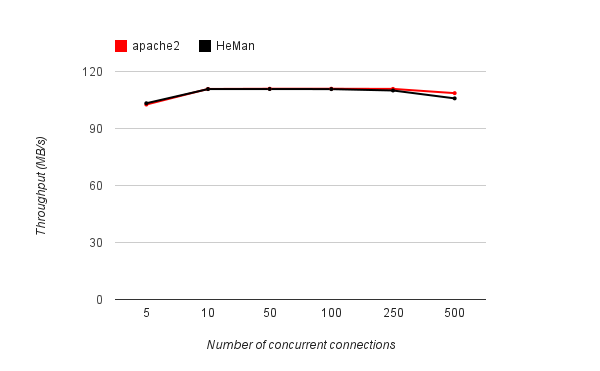
\includegraphics[width=0.9\textwidth]{128kb_graph.png}
	\caption{Web server benchmark, 128kb file}
	\label{fig:graph128}
\end{figure*}
\begin{figure*}[!htb]
	\centering
	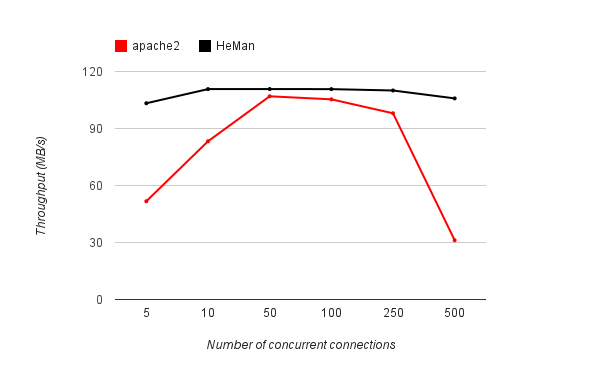
\includegraphics[width=0.9\textwidth]{16kb_graph.png}
	\caption{Web server benchmark, 16kb file}
	\label{fig:graph16}
\end{figure*}


\subsection{Memory Overhead}

The per-thread memory overhead imposed by He-Man is very small: it
consists of a thread id, list pointers for the scheduling queue, the
next state to enter, a pointer to the most recently received event,
and list heads and tails for lists of the events being waited on,
events owned by the thread, and buffers owned by the thread (the
latter two are so that we can automatically reclaim these resources
when the thread exits). On a 64-bit system, the total overhead comes
out to 88 bytes, and could easily be reduced further (e.g. by using
singly linked lists).  For comparison, the default thread stack size
under NPTL on Linux is 2 megabytes.

% see how many threads we can spawn with Memory.hs

\section{Future work}

We will continue our work on He-Man, and hope to submit it to a programming
languages conference such as ICFP. We plan to expand the language with the
ability to declare functions and make non-external function calls within a
thread. This will make code simpler and shorter by allowing the programmer to
abstract away common functionality like read and write loops.

In the runtime, our current thread \t{struct}s are larger than necessary.
Because the runtime allocates a \t{struct} on every thread spawn, we should
replace our \t{malloc} calls with calls to a custom slab allocator. We also plan
on writing a multithreaded runtime, to allow servicing multiple threads' ready
events simultaneously. Because our threads don't interact, this does not require
exposing any locking to the programmer.

The backend can perform more aggressive optimization on the code blocks. In
particular, we currently do not allow any control flow except at tail position;
if both branches of an \t{if} are non-blocking, we should avoid translating it
into multiple blocks, requiring a yield to the main loop. It should also be
possible to gather interesting output from the backend, like a graphical
representation of the generated state machine, for documentation purposes.

We also hope to implement observable sharing, as in \cite{Gill}, to allow the
same thread to have distinct spawn sites without code duplication. This does not
add inefficiency, but does increase the size of our output code. 

\section{Conclusions}

\bibliography{citations}{}
\bibliographystyle{abbrvnat}

\end{document}
